\documentclass{article}
\usepackage{eecstex}
\usepackage{physics}
\usepackage{pgfplots}

\renewcommand{\thesubsection}{\thesection.\arabic{subsection}}
\renewcommand{\thesubsubsection}{\thesubsection.\alph{subsubsection}}
\renewcommand{\labelenumi}{\arabic{enumi}.}
\newcommand{\F}{\mathcal{F}}

\title{EE 120 HW 04}
\author{Bryan Ngo}
\date{2021-02-19}

\begin{document}

\maketitle

\section{Continuous Time Fourier Transform}

\begin{enumerate}
    \item \(\F\{\delta(t - 5)\} = \int_{\R} \delta(t - 5) e^{-j \omega t} \, dt = e^{-5j \omega}\)
    \item \(\F\{e^{-at} u(t)\} = \int_0^\infty e^{-t (a + j \omega)} \, dt = \frac{1}{a + j \omega}\)
    \item \(\F\{e^{(-1 + 2j) t}\} = \frac{1}{-1 + 2j + j \omega} = \frac{1}{1 + (2 + \omega) j}\)
\end{enumerate}
Plotting the Fourier tranforms,
\begin{center}
    \begin{tikzpicture}
        \begin{axis}[
            xlabel=\(\omega\), ylabel={\(|\F\{\delta(t - 5)\}|\)},
            axis lines=middle,
            ymin=0, ymax=1.5
        ]
        \addplot[
            color=blue,
            domain=-5:5
        ]{1};
        \end{axis}
    \end{tikzpicture}
    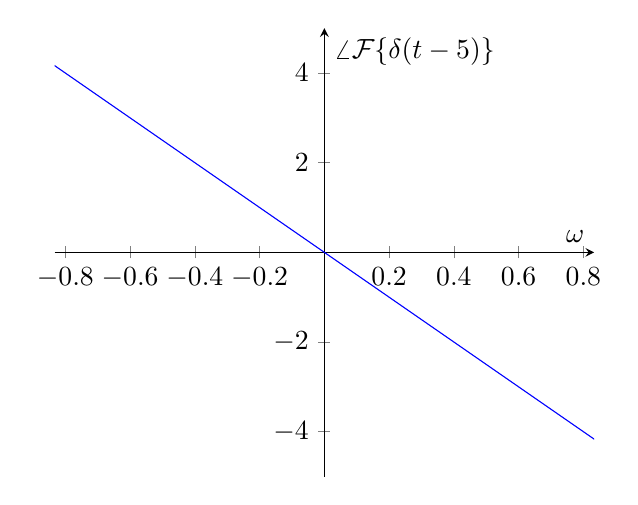
\begin{tikzpicture}
        \begin{axis}[
            xlabel=\(\omega\), ylabel={\(\angle\F\{\delta(t - 5)\}\)},
            axis lines=middle,
            ymin=-5, ymax=5
        ]
        \addplot[
            color=blue,
            domain=-5:5
        ]{-5*x};
        \end{axis}
    \end{tikzpicture}
    \begin{tikzpicture}
        \begin{axis}[
            xlabel=\(\omega\), ylabel={\(|\F\{e^{-at} u(t)\}|\) (\(a = 1\))},
            axis lines=middle,
            ymin=0, ymax=1.5,
        ]
        \addplot[
            color=blue,
            domain=-5:5,
            samples=200
        ]{1 / sqrt(1 + x^2)};
        \end{axis}
    \end{tikzpicture}
    \begin{tikzpicture}
        \begin{axis}[
            xlabel=\(\omega\), ylabel={\(\angle\F\{e^{-at} u(t)\}\) (\(a = 1\))},
            axis lines=middle,
            ymin=-5, ymax=5
        ]
        \addplot[
            color=blue,
            domain=-5:5
        ]{rad(atan(-x))};
        \end{axis}
    \end{tikzpicture}
    \begin{tikzpicture}
        \begin{axis}[
            xlabel=\(\omega\), ylabel={\(|\F\{e^{(-1 + 2j) t} u(t)\}|\)},
            axis lines=middle,
            ymin=0, ymax=1.5,
        ]
        \addplot[
            color=blue,
            domain=-5:5,
            samples=200
        ]{1 / sqrt(1 + (2 + x)^2)};
        \end{axis}
    \end{tikzpicture}
    \begin{tikzpicture}
        \begin{axis}[
            xlabel=\(\omega\), ylabel={\(\angle\F\{e^{(-1 + 2j) t} u(t)\}\)},
            axis lines=middle,
            ymin=-5, ymax=5
        ]
        \addplot[
            color=blue,
            domain=-5:5
        ]{rad(atan(-(2 + x)))};
        \end{axis}
    \end{tikzpicture}
\end{center}

\section{Fourier Transform of a Gaussian Signal}

\begin{align}
    X(\omega) &= \int_{\R} e^{-t^2} e^{-j \omega t} \, dt \\
    X(0) &= \sqrt{\pi}
\end{align}

\subsection{}

\begin{equation}
    \diff{\omega} X(\omega) = \frac{j}{2} \int_{\R} \diff{t} (e^{-t^2}) e^{-j \omega t} \, dt
\end{equation}
Letting \(u = e^{-j \omega t} \implies du = -j \omega e^{-j \omega t} \, dt\) and \(dv = \diff{t} e^{-t^2} \, dt \implies v = e^{-t^2}\),
\begin{align}
    \diff{\omega} X(\omega) &= \eval{\frac{j}{2} e^{-t^2} e^{-j \omega t}}_{\R} - \frac{\omega}{2} \int_{\R} e^{-t^2} e^{-j \omega t} \, dt \\
    &= \cancelto{0}{\eval{\frac{j}{2} e^{-t^2} e^{-j \omega t}}_{\R}} - \frac{\omega}{2} X(\omega) = \frac{\omega}{2} X(\omega)
\end{align}

\subsection{}

\begin{align}
    \diff{\omega} \alpha e^{-\frac{1}{\beta} \omega^2} &= -\frac{2 \alpha \omega}{\beta} e^{-\frac{1}{\beta} \omega^2} \\
    -\frac{\omega}{2} \alpha e^{-\frac{1}{\beta} \omega^2} &= -\frac{\alpha \omega}{2} e^{-\frac{1}{\beta} \omega^2}
\end{align}
Meaning that \(\beta = 4\).
Solving for the initial condition, we get that \(\alpha = \sqrt{\pi}\).

\section{Frequency Response}

\begin{align}
    h(t) &= \delta(t - 2) \\
    g(t) &= e^{-\alpha |t|}
\end{align}

\subsection{}

\begin{align}
    H(\omega) &= e^{-2j \omega} \\
    G(\omega) &= \int_{\R} e^{-\alpha |t|} e^{-j \omega t} \, dt \\
    &= \int_{-\infty}^0 e^{\alpha t} e^{-j \omega t} + \int_0^\infty e^{-\alpha t} e^{-j \omega t} \, dt = \frac{1}{\alpha - j\omega} + \frac{1}{\alpha + j\omega}
\end{align}

\subsection{}

\begin{align}
    s_1(t) &= h(t) \ast g(t) = e^{-\alpha |t - 2|} \\
    s_2(t) &= h(t) + g(t) = \delta(t - 2) + e^{-\alpha |t|} \\
    S_1(\omega) &= H(\omega) G(\omega) = \qty(\frac{1}{\alpha - j \omega} + \frac{1}{\alpha + j \omega}) e^{-2j \omega} \\
    S_2(\omega) &= H(\omega) + H(\omega) = \frac{1}{\alpha - j \omega} + \frac{1}{\alpha + j \omega} + e^{-2j \omega}
\end{align}

\section{Fourier Series}

\begin{align}
    x_1(t) &= 1 + \sin(\frac{2 \pi t}{10}) \\
    x_2(t) &= 1 + \sin(\frac{5 \pi}{3} t + \frac{\pi}{2}) \\
    x_3(t) &= x_1(t) + x_2(t) \\
    x(t) &= \sum_{k \in \Z} a_k e^{j k \omega_0 t}
\end{align}

\subsection{}

We have \(T_1 = 10\), \(T_2 = \frac{6}{5}\), \(T_3 = \operatorname{lcm}(T_1, T_2) = 30\).

\subsection{}

Transforming into complex exponentials,
\begin{align}
    x_1(t) &= 1 + \frac{1}{2j} (e^{j\frac{\pi}{5} t} - e^{-j\frac{\pi}{5} t}) = -\frac{1}{2j} e^{-j \frac{\pi}{5} t} + 1 + \frac{1}{2j} e^{j \frac{\pi}{5} t} \\
    \implies a_{1k} &=
    \begin{cases}
        -\frac{1}{2j} & k = -1 \\
        1 & k = 0 \\
        \frac{1}{2j} & k = 1 \\
        0 & \text{otherwise}
    \end{cases} \\
    x_2(t) &= 1 + \frac{e^{\frac{pi}{2}}}{2j} (e^{j \frac{5 \pi}{3} t} - e^{-j \frac{5 \pi}{3} t}) = -\frac{e^{\frac{\pi}{2}}}{2j} e^{-j \frac{5 \pi}{3} t} + 1 + \frac{e^{\frac{\pi}{2}}}{2j} e^{j \frac{5 \pi}{3} t} \\
    \implies a_{2k} &=
    \begin{cases}
        -\frac{e^{\frac{\pi}{2}}}{2j} & k = -1 \\
        1 & k = 0 \\
        \frac{e^{\frac{\pi}{2}}}{2j} & k = 1 \\
        0 & \text{otherwise}
    \end{cases} \\
    \implies a_{3k} &=
    \begin{cases}
        -\frac{1}{2j} (e^{\frac{\pi}{2}} + 1) & k = -1 \\
        2 & k = 0 \\
        \frac{1}{2j} (e^{\frac{\pi}{2}} + 1) & k = 1 \\
        0 & \text{otherwise}
    \end{cases}
\end{align}
where we determined \(a_{3k}\) through the linearity of the CTFS.

\section{Ideal Low-Pass Filter}

\begin{equation}
    H(\omega) =
    \begin{cases}
        1 & |\omega| < \alpha \\
        0 & \text{elsewhere}
    \end{cases}
\end{equation}

\subsection{}

\begin{align}
    h(t) &= \frac{1}{2 \pi} \int_{\R} H(\omega) e^{j \omega t} \, d\omega \\
    &= \frac{1}{2 \pi} \int_{-\alpha}^\alpha e^{j \omega t} \, d\omega = \frac{1}{2 \pi j t} \eval{e^{j \omega t}}_{-\alpha}^\alpha = \frac{1}{2 \pi jt} (e^{j \alpha t} - e^{-j \alpha t}) = \frac{1}{\cancel{2j} \pi t} (\cancel{2j} \sin(\alpha t)) = \frac{\alpha}{\pi} \operatorname{sinc}(\alpha t)
\end{align}

\subsection{}

\subsubsection{}

From lecture, the CTFS of any periodic function can be expressed as
\begin{equation}
    x(t) = \frac{1}{T} \sum_{k \in \Z} G\qty(\frac{k}{T}) e^{\frac{k}{T} j 2 \pi t}
\end{equation}
where \(G(\frac{k}{T})\) is the \(a_k\) coefficients represented by the CTFT of one period of the function.
Since one period of the comb function is simply a delta function, \(a_k = \frac{1}{T}\) for all \(k\).

\subsubsection{}

Plugging \(a_k\) into the formula for \(X(\omega)\),
\begin{equation}
    X(\omega) = \frac{2\pi}{T} \sum_{k \in \Z} \delta\qty(\omega - \frac{2\pi k}{T})
\end{equation}
Meaning that
\begin{equation}
    Y(\omega) = H(\omega) X(\omega) = \frac{2\pi}{T} \sum_{k \in [-2, 2]} \delta\qty(\omega - \frac{2\pi k}{T})
\end{equation}
since the only acceptable values of \(k\) such that \(\qty|\omega - \frac{2\pi k}{T}| < \alpha\) are the interval \([-2, 2]\).

\subsubsection{}

\begin{align}
    y(t) &= \frac{1}{2\pi} \int_{\R} \frac{2\pi}{T} \sum_{k \in [-2, 2]} \delta\qty(\omega - \frac{2\pi k}{T}) e^{j \omega t} \, d\omega \\
    &= \frac{1}{T} \sum_{k \in [-2, 2]} \int_{\R} \delta\qty(\omega - \frac{2\pi k}{T}) e^{j \omega t} \, d\omega \\
    &= \frac{1}{T} \sum_{k \in [-2, 2]} e^{j \frac{2\pi k}{T} t} = \frac{1}{T} (1 + e^{j \frac{2\pi}{T} t} + e^{-j \frac{2\pi}{T} t} + e^{2j \frac{2\pi}{T} t} + e^{-2j \frac{2\pi}{T} t}) \\
    &= \frac{1}{T} \qty(1 + 2\cos(\frac{2\pi}{T} t) + 2\cos(\frac{4\pi}{T} t))
\end{align}

\subsubsection{}

\begin{center}
    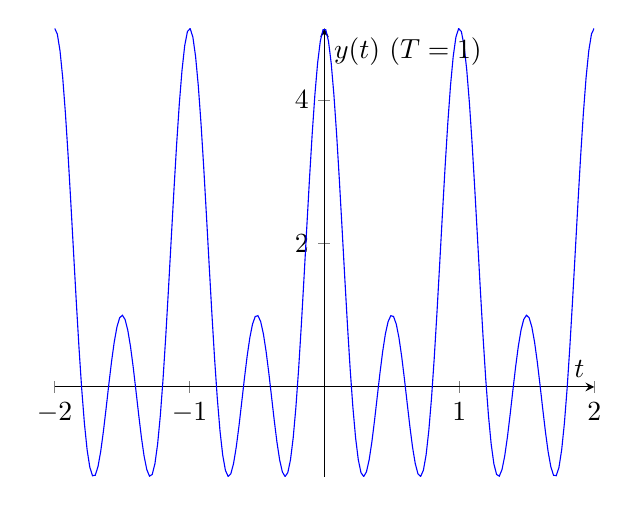
\begin{tikzpicture}
        \begin{axis}[
            xlabel=\(t\), ylabel={\(y(t)\) (\(T = 1\))},
            axis lines=middle,
        ]
        \addplot[
            color=blue,
            domain=-2:2,
            samples=200
        ]{1 + 2*cos(2*pi*deg(x)) + 2*cos(4*pi*deg(x))};
        \end{axis}
    \end{tikzpicture}
\end{center}
Essentially, the low pass filter "blurs" the original comb function, spreading it out.
This is because the low pass filter eliminates all frequencies after a certain cutoff.
Note the peaks of where the original comb function are which line up with that of \(y(t)\).

\end{document}
